\documentclass[12pt,aspectratio=169]{beamer}

%
\usepackage{algorithm,algorithmic}
%
%\usepackage[utf8]{inputenc}
%\usepackage{booktabs}
%\usepackage[opacity=0.1]{pdfcomment} % set to 0 to make annotation icons invisible
%\usepackage{pdfpc}
%\usepackage{arev}
%\usepackage{multicol}
%
%\usepackage{xcolor, color, colortbl}
%\definecolor{dkgreen}{rgb}{0,0.5,0}
%\definecolor{dkred}{rgb}{0.8,0,0}
%\definecolor{dkblue}{rgb}{0,0,0.5}
%\definecolor{gray}{rgb}{0.5,0.5,0.5}
%\definecolor{mauve}{rgb}{0.58,0,0.82}
%\definecolor{hilight}{RGB}{122,86,0}
%
%\definecolor{LRed}{rgb}{1,.8,.8}
%\definecolor{MRed}{rgb}{1,.6,.6}
%\definecolor{HRed}{rgb}{1,.2,.2}
%
%%Information to be included in the title page:
%
%\tikzset{
%        ->,  % makes the edges directed
%        >=stealth', % makes the arrow heads boldnode 
%        distance=3cm, % specifies the minimum distance between two nodes. Change if necessary.
%        every state/.style={thick, fill=gray!10}, % sets the properties for each ’state’ node
%        initial text=$ $, % sets the text that appears on the start arrow
%}
%
%\def\firstcircle{(90:1.75cm) circle (2cm)}
%\def\secondcircle{(210:1.75cm) circle (2cm)}
%\def\thirdcircle{(330:1.75cm) circle (2cm)}
%
%\usepackage{tikz}
%\usetikzlibrary{arrows.meta,
%                calc, chains,
%                quotes,
%                positioning,
%                shapes.geometric}
%
%
%\def\scalefact{0.85}
%\newcommand{\cev}[1]{\reflectbox{\ensuremath{\vec{\reflectbox{\ensuremath{#1}}}}}}
%\newcommand{\evalat}[2]{\left.#1\right\vert_{#2}}
%
%\newcommand{\znode}[5][black]{\path (#3,#4) node(#2) [circle,draw,color=#1] {#5};}
%\newcommand{\zunedge}[6][black]{%
%\begin{scope}
%	\path (#2,#3) node(this) [inner sep=0pt,triangle,draw,color=#1] {#4};
%	\draw[->,color=#1] (#5) -- (this.west);
%	\draw[->,color=#1] (this.east) -- (#6);
%\end{scope}}
%\newcommand{\zbiedge}[7][black]{%
%\begin{scope}
%	\path (#2,#3) node(this) [inner sep=0pt,triangle,draw,color=#1] {#4};
%	\draw[->,color=#1] (#5) -- (this);
%	\draw[->,color=#1] (#6) -- (this);
%	\draw[->,color=#1] (this.east) -- (#7);
%\end{scope}}
%\newcommand{\zedge}[5][black]{\path (#3,#4) node(#2) [inner sep=0pt,triangle,draw,color=#1] {#5};}
%
%\definecolor{blue(pigment)}{rgb}{0.2, 0.2, 0.6}
%\definecolor{burgundy}{rgb}{0.5, 0.0, 0.13}
%
%
%\usepackage{listings}
%%% \usetheme{Goettingen}
%\usefonttheme{serif}
%\usepackage{times}
%\setbeamertemplate{navigation symbols}{}
%
%\title{Perceptron}
% 
% 
%%\author[Mehrdad Maleki] % (optional, for multiple authors)
%%{Mehrdad Maleki, Barak A. Pearlmutter\footnote{ Institute & Department of Computer Science
%%Maynooth University, Co. Kildare, Ireland}, Jeffrey Mark Siskind}
% 
%%\institute[NUIM] % (optional)
%%{
%%  Department of Computer Science \\
%%  National University of Ireland Maynooth
% 
%%}


\usepackage[utf8]{inputenc}
%\usepackage[table]{xcolor}
\usepackage{color, colortbl}
\definecolor{LRed}{rgb}{1,.8,.8}
\definecolor{MRed}{rgb}{1,.6,.6}
\definecolor{HRed}{rgb}{1,.2,.2}
\usepackage{tikz}
\definecolor{Gray}{gray}{0.9}
\definecolor{Green}{rgb}{0.3,0.9,0.3}
\definecolor{Red}{rgb}{0.98,0.3,0.3}
\usetikzlibrary{automata, positioning, arrows}
%Information to be included in the title page:

\tikzset{
        ->,  % makes the edges directed
        >=stealth', % makes the arrow heads boldnode 
        distance=3cm, % specifies the minimum distance between two nodes. Change if necessary.
        every state/.style={thick, fill=gray!10}, % sets the properties for each ’state’ node
        initial text=$ $, % sets the text that appears on the start arrow
}

\usepackage{tkz-euclide}

\usepackage{multimedia}

\def\firstcircle{(90:1.75cm) circle (2cm)}
\def\secondcircle{(210:1.75cm) circle (2cm)}
\def\thirdcircle{(330:1.75cm) circle (2cm)}

%\usetheme{Madrid}

\title[Finite Automata] %optional
{Deep Learning}
 
\subtitle{Lecture 2: Probability Theory}
 
%\author[Maleki] % (optional, for multiple authors)
%{Mehrdad Maleki}
% 
%\institute[NUIM] % (optional)
%{
%  Department of Computer Science \\
%  National University of Ireland Maynooth
% 
%}
 
\date{February 2020}

\author[]{\textbf{Dr. Mehrdad Maleki}}

%\author[]{\textbf{Mehrdad Maleki}\textsuperscript{1}}
%\institute[]{\textsuperscript{1}Department of Computer Science\\ National University of Ireland\\ Maynooth}
 
\date{}
 
%\logo{\includegraphics[height=1.5cm]{lion-logo.png}}

\renewcommand{\Re}{\mathbb{R}}
 
\begin{document}
 
\frame{\titlepage}

\newcommand{\SYSTEM}[2]{\raisebox{-1ex}{\shortstack{#1\\[-0.25ex]\tiny #2}}}
\newcommand{\YES}{\textcolor{dkgreen}{$\ballotcheck$}}
\newcommand{\NOPE}{\textcolor{dkred}{$\ballotx$}}
\newcommand{\MAYBE}{\textcolor{dkblue}{\textbf{?}}}


\begin{frame}
\frametitle{Random Variable}
A \textbf{random variable} is a variable whose values are depend on the outcome of a random event. \pause
Let $\mathbf{X}$ be the outcomes of tossing a coin, then if Head appears $\mathbf{X}=1$ and if Tails appears $\mathbf{X}=0$. \pause $\mathbf{X}$ could be the outcome of tossing a dice, in this case $\mathbf{X}\in \{1,2,3,4,5,6\}$. $\mathbf{X}$ could be the height of people comming to a bank. \pause The set of all possible outputs of a random variable is called the sample space of that random variable and usually we denote it by $S$. \pause In fact any subset of the sample space is the random event.

\end{frame}


\begin{frame}
\frametitle{Probability}
In tossing a coin we can ask question like "How likely is that the value of $\mathbf{X}$ is equal 1?".\pause This is the probability of the events that for them $\mathbf{X}=1$.\pause This is a real number between $0$ and $1$ and we denote this by $P[\mathbf{X}=1]$ 
\end{frame}

\begin{frame}
If $S$ be a finite set then probability of event $A\subseteq S$ is define as follow,
\[
P(A)=P(\mathbf{X}\in A)=\frac{|A|}{|S|}
\]
\end{frame}

\begin{frame}
\[
\begin{aligned}
& 0\leq P(A) \leq 1\\ \pause
& P(\emptyset)=0\\ \pause
& P(S)=1\\ \pause
& \textbf{if } A\cap B=\emptyset \Rightarrow P(A\cup B)=P(A)+P(B)
\end{aligned}
\]
\end{frame}


\begin{frame}
\frametitle{Discerete Distribution}
A discrete random variable has a countable number of possible values.\pause\\
\textbf{Probability function}: describe the probability $P(\mathbf{X}\in A)$ that $A$ is a random event from the sample space.\pause\\
\textbf{Probability mass function (pmf)}: $f(i)=P[\mathbf{X}=i]$ for descrete random variables.

\end{frame}


\begin{frame}
\frametitle{Continious Distribution}
In general, quantities such as pressure, height, mass, weight, density, volume, temperature, and distance are examples of continuous random variables. \pause Between any two values of a continuous random variable, there are an infinite number of other valid values.
\end{frame}

\begin{frame}
\textbf{Probability density function (pdf)}: Is a continuous positive function $f_{\mathbf{X}}(x):\Re\to \Re^{\geq 0}$ such that,\pause
\[
\int_{-\infty}^{\infty}f_{\mathbf{X}}(x)dx=1
\]\pause
\begin{center}
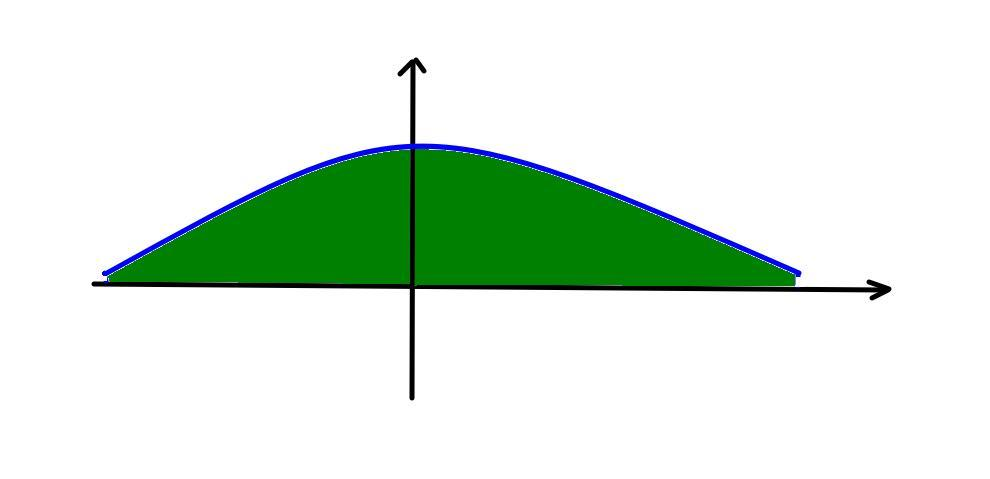
\includegraphics[scale=0.4]{normal}
\end{center}
\end{frame}


\begin{frame}
\textbf{Cumulative distribution function}: is the function that evaluating the probability of $\mathbf{X}\leq x$,\pause i.e., $F_{\mathbf{X}}(x)=P[\mathbf{X}\leq x]$ \pause
\begin{center}
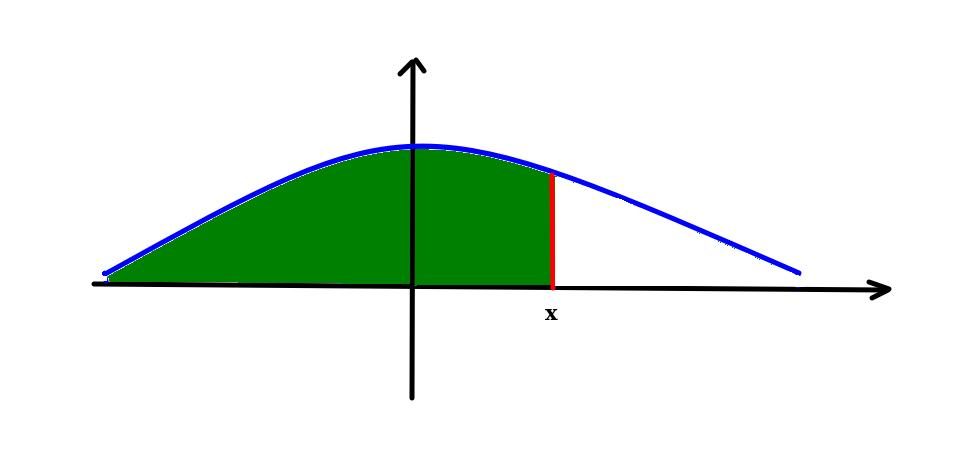
\includegraphics[scale=0.4]{normal2}
\end{center}
\end{frame}


\begin{frame}
\frametitle{Bernoulli Trial}
A \textbf{Bernoulli trial} is a random experiment with exactly two possible outcomes, "success" and "failure". \pause
\[
\begin{aligned}
&p=P[\mathbf{X}="success"]\\ \pause
&q=P[\mathbf{X}="failure]\\ \pause
&p+q=1
\end{aligned}
\]
\end{frame}

\begin{frame}
Probability mass function (PMF) of Bernouli distribution,\pause
\[
\begin{aligned}
&f(x=0|\mathbf{p})=q\\ \pause
&f(x=1|\mathbf{p})=p
\end{aligned}
\] \pause
where $\mathbf{p}=(p,q)$. So,\pause
\[
\begin{aligned}
f(x|\mathbf{p})&=p^xq^{1-x}\\ \pause
&=p^x(1-p)^{1-x}
\end{aligned}
\]\pause
for $x\in \{0,1\}$.
\end{frame}




\begin{frame}
\frametitle{Categorical (generalized Bernoulli) Distribution}
\textbf{Categorical distribution} is a discrete probability distribution that describes the possible results of a random variable that can take on one of $K$ possible categories, with the probability of each category separately specified. So $\mathbf{X}\in\{1,2,\dots,K\}$.
\end{frame}


\begin{frame}
Probability mass function (PMF) of Categorical distribution,\pause
\[
\begin{aligned}
&f(x=i|\mathbf{p})=p_i\\
\end{aligned}
\] \pause
where $\mathbf{p}=(p_1,\dots,p_K)$. So,\pause
\[
\begin{aligned}
f(x|\mathbf{p})&=p_1^{\mathbf{I}_{[x=1]}}\dots p_K^{\mathbf{I}_{[x=K]}} \\ \pause
&=\prod_{i=1}^K\,p_i^{\mathbf{I}_{[x=i]}}
\end{aligned}
\]\pause
where
\[
\mathbf{I}_{[x=i]}=
\left\{ \begin{array}{cc}
1 & \mbox{if $x=i$}\\
0 & \mbox{else}
\end{array} \right.
\]
for $x\in \{0,1\}$.
\end{frame}



\begin{frame}
\frametitle{Conditional Probability}
Conditional probability is a measure of the probability of an event occurring, given that another event (by assumption, presumption, assertion or evidence) has already occurred.\pause  The conditional probability of $A$ given $B$ is defined as follow,
\[
P(A|B)=\frac{P(A\cap B)}{P(B)}
\]
\end{frame}

\begin{frame}
\begin{center}
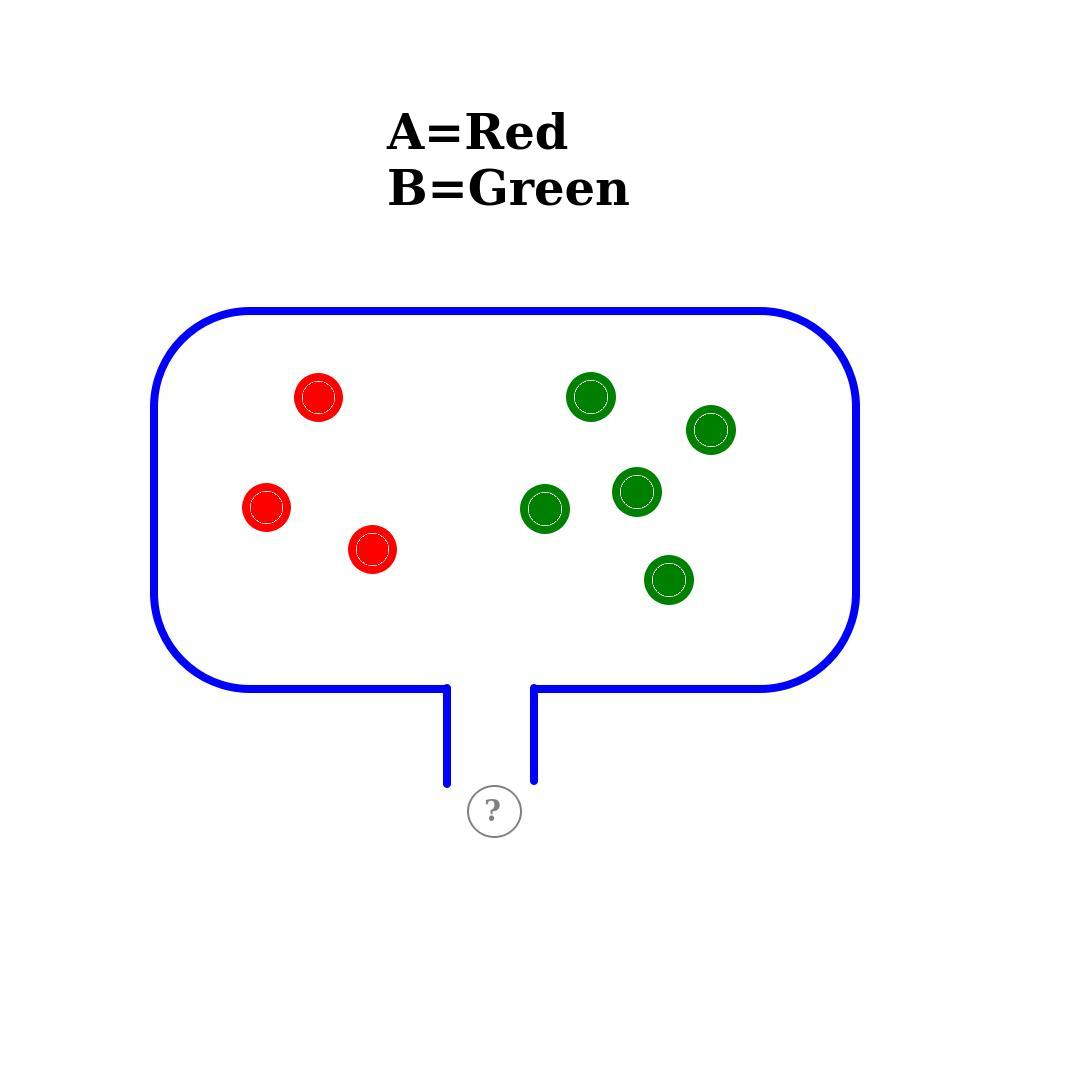
\includegraphics[scale=0.2]{balls}
\end{center}\pause
We choose one ball randomly. What is the probability that this ball is red?
\pause $P(A)=\frac{3}{8}$, \pause What about the probability that this ball is green?\pause $P(B)=\frac{5}{8}$.

\end{frame}


\begin{frame}
\begin{center}
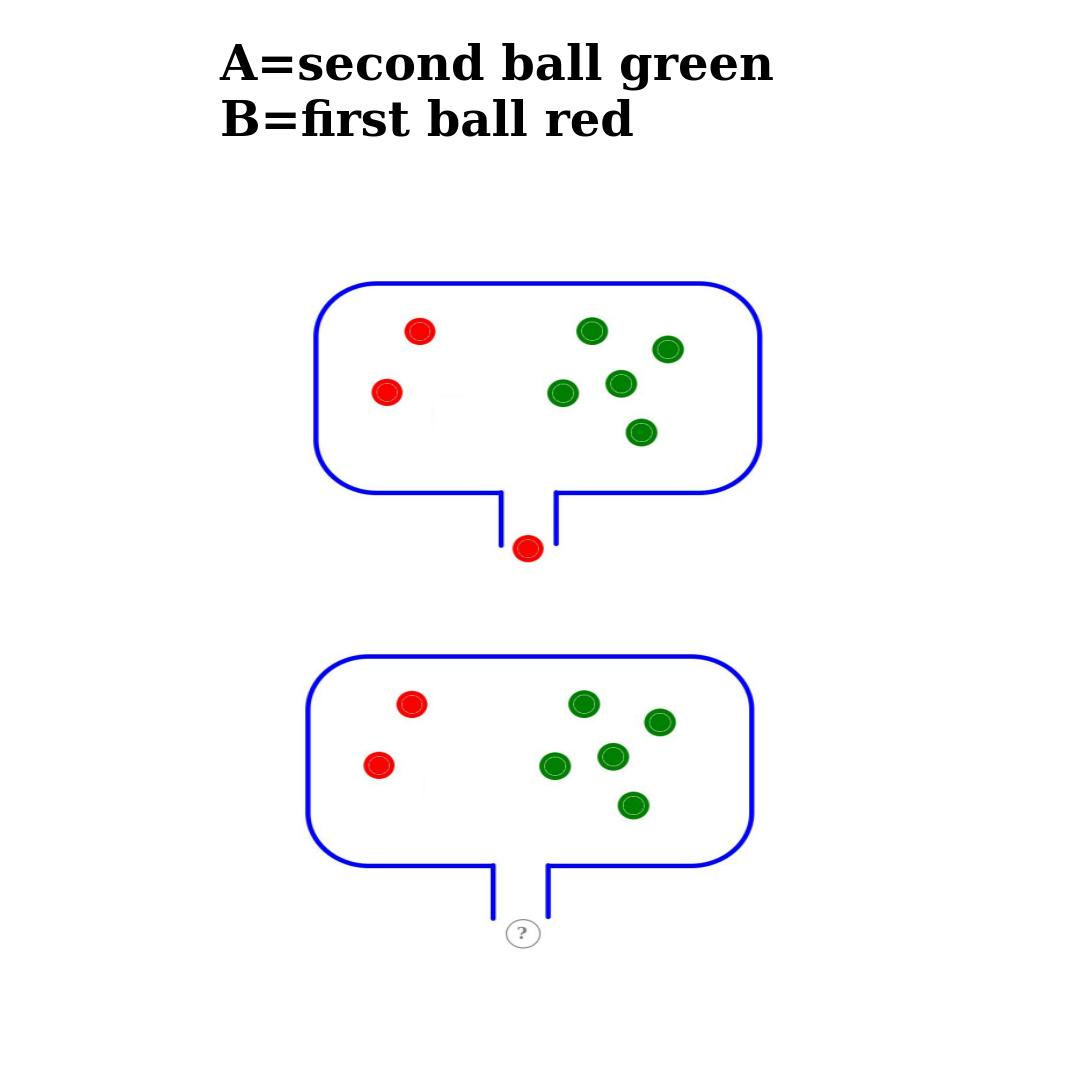
\includegraphics[scale=0.23]{balls2}
\end{center}\pause
We choose one ball randomly and through it away. We choose another ball randomly. What is the probability that the second ball is green such that the fist ball is red?\pause $P(A|B)=\frac{5}{7}$

\end{frame}

\begin{frame}
\frametitle{Law of Total Probability}
\begin{center}
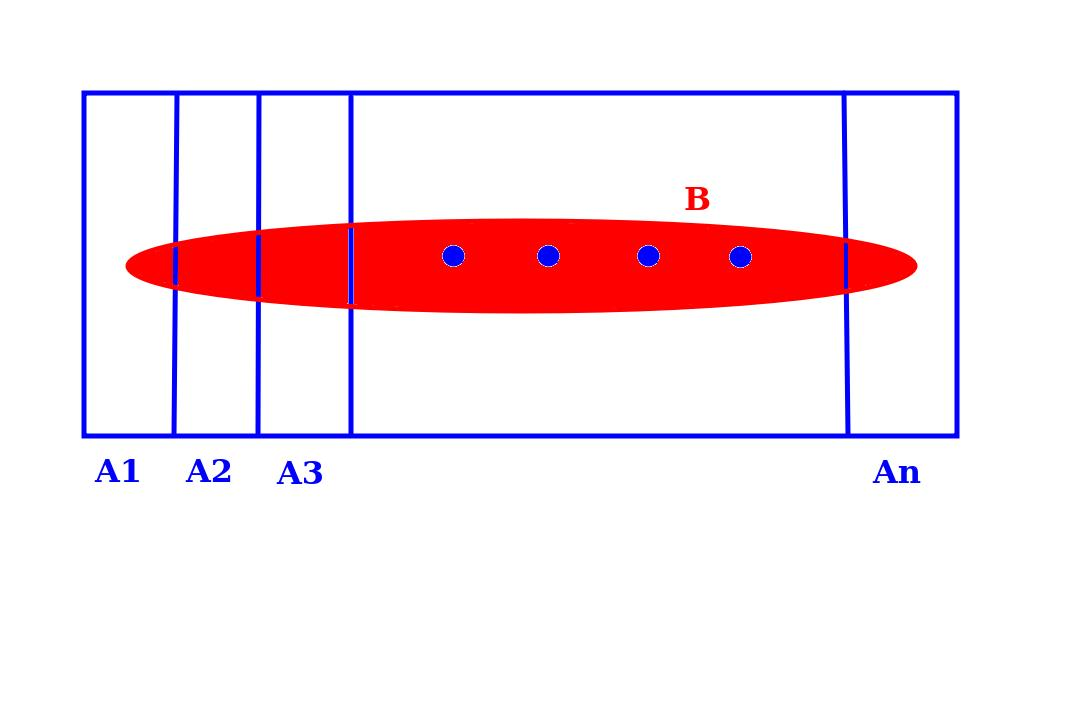
\includegraphics[scale=0.25]{balls4}
\end{center}\pause
\[
\begin{aligned}
P(B)&=P(A_1\cap B)+\dots +P(A_n\cap B)\\ \pause
&=P(A_1)P(B|A_1)+\dots+P(A_n)P(B|A_n)
\end{aligned}
\]
\end{frame}


\begin{frame}
\begin{center}
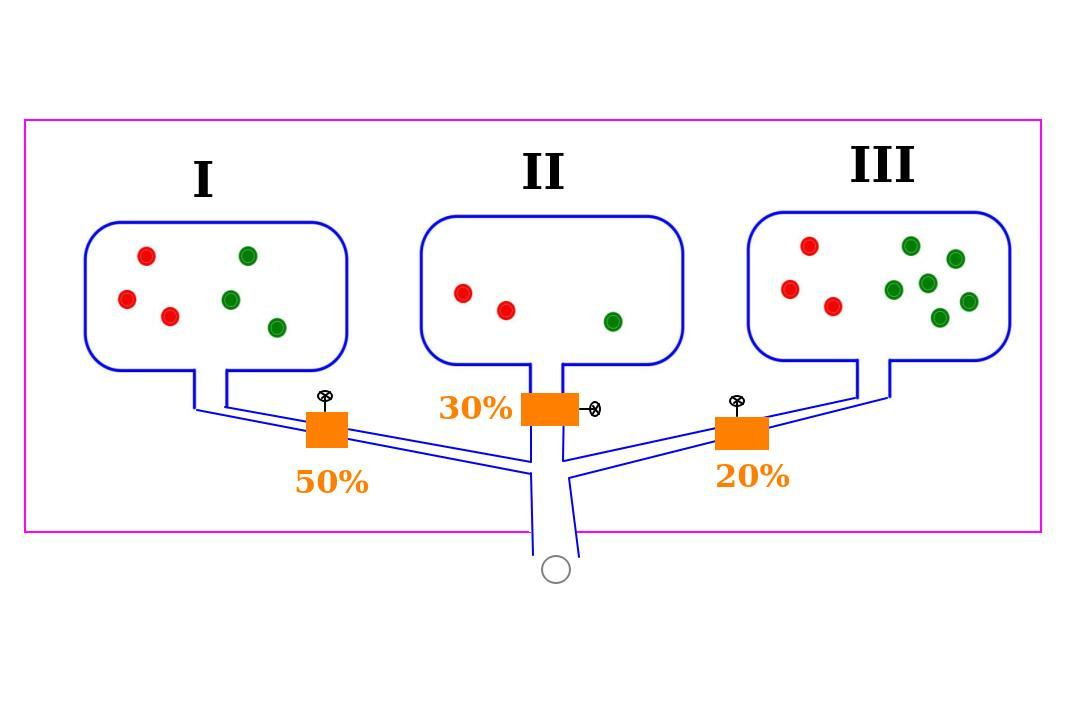
\includegraphics[scale=0.3]{balls3}
\end{center}
\[
\begin{aligned}
P(R)&=\pause P(I)P(R|I)+P(II)P(R|II)+P(III)P(R|III)\\ \pause
&= 0.5\frac{3}{6}+0.3\frac{2}{3}+0.2\frac{3}{9}\\ \pause
&\approx 0.52
\end{aligned}
\]

\end{frame}


\begin{frame}
\begin{center}
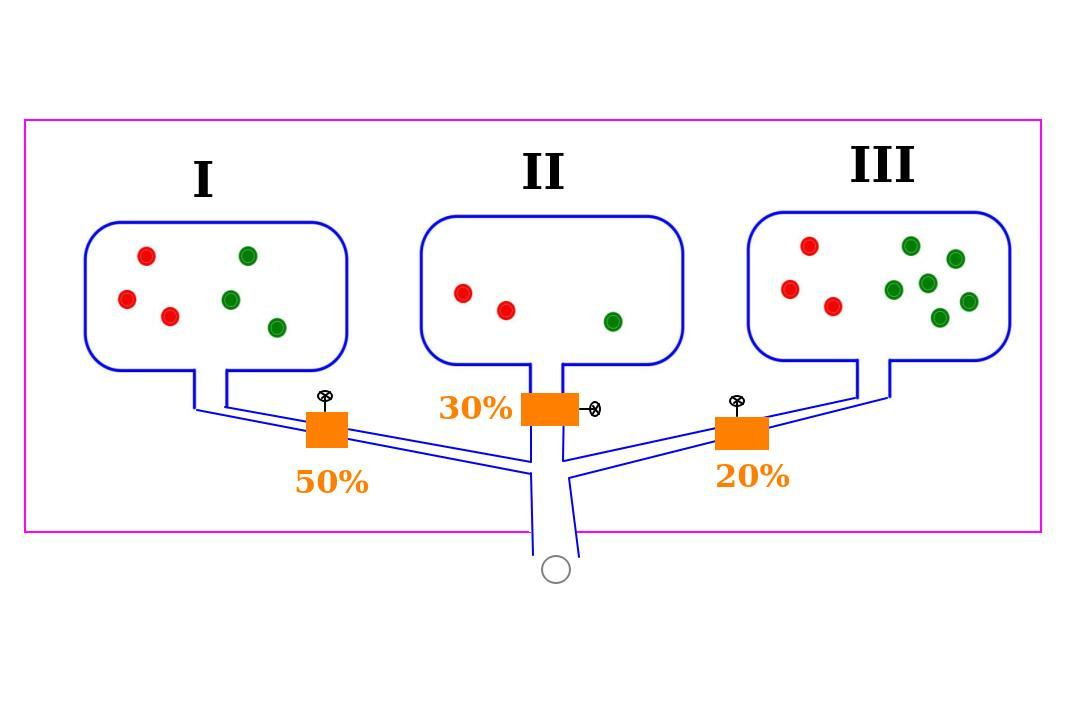
\includegraphics[scale=0.3]{balls3}
\end{center}
\[
\begin{aligned}
P(G)&=\pause P(I)P(G|I)+P(II)P(G|II)+P(III)P(G|III)\\ \pause
&= 0.5\frac{3}{6}+0.3\frac{1}{3}+0.2\frac{6}{9}\\ \pause
&\approx 0.48
\end{aligned}
\]

\end{frame}


\begin{frame}
\frametitle{Motivation- Thinking Fast and Slow}
\framesubtitle{(Daniel Kahneman)}\pause
A cab was involved in a hit-and-run accident at night.\pause Two cab companies, the Green and the Blue, operate in the city. \pause You are given the following data: \pause $85\%$ of the cabs in the city are Green and $15\%$ are Blue. \pause  A witness identified the cab as Blue. \pause The court tested the reliability of the witness under the circumstances that existed on the night of the accident \pause  and concluded that the witness correctly identified each one of the two colors $80\%$ of the time and failed $20\%$ of the time. \pause  What is the probability that the cab involved in the accident was Blue rather than Green?
\end{frame}

\begin{frame}
\frametitle{Bayes Rule}
Bayes' theorem links the degree of belief in a proposition before and after accounting for evidence, \pause
\[
P(A|B)=\frac{P(B|A)P(A)}{P(B)}
\]\pause
\begin{itemize}
\item $P(A)=$ \textbf{the prior}, is the initial degree of belief in $A$.\pause
\item $P(A|B)=$ \textbf{the posterior}, is the degree of belief after incorporating news that $B$ is true.\pause
\item $P(B|A)=$ \textbf{the likelihood}, that can be estimated from the training data. 
\end{itemize}
\end{frame}

\begin{frame}
\begin{center}
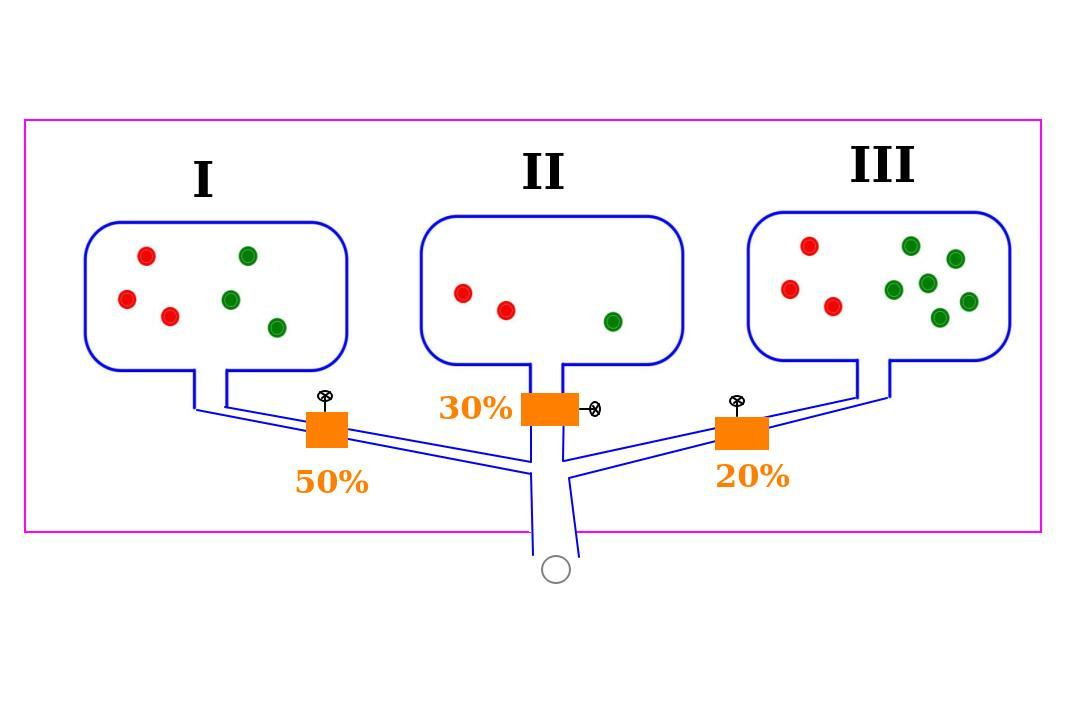
\includegraphics[scale=0.3]{balls3}
\end{center}
\[
\begin{aligned}
P(I|R)&=\pause \frac{P(R|I)P(I)}{P(R)}\\
&=\frac{\frac{3}{6}0.5}{0.52}\\
& \approx 0.48
\end{aligned}
\]
\end{frame}


\begin{frame}
\[
\begin{aligned}
P(II|R)&=\pause \frac{P(R|II)P(II)}{P(R)}\\
&=\frac{\frac{2}{3}0.3}{0.52}\\
& \approx 0.38
\end{aligned}
\]
\[
\begin{aligned}
P(III|R)&=\pause \frac{P(R|III)P(III)}{P(R)}\\
&=\frac{\frac{3}{9}0.2}{0.52}\\
& \approx 0.12
\end{aligned}
\]
\end{frame}


\begin{frame}
\[
\begin{aligned}
P(I|G)&=\pause \frac{P(G|I)P(I)}{P(G)}\\
&=\frac{\frac{3}{6}0.5}{0.48}\\
& \approx 0.52
\end{aligned}
\]
\[
\begin{aligned}
P(II|G)&=\pause \frac{P(G|II)P(II)}{P(G)}\\
&=\frac{\frac{1}{3}0.3}{0.48}\\
& \approx 0.2
\end{aligned}
\]
\[
\begin{aligned}
P(III|G)&=\pause \frac{P(G|III)P(III)}{P(G)}\\
&=\frac{\frac{6}{9}0.2}{0.48}\\
& \approx 0.27
\end{aligned}
\]
\end{frame}


\begin{frame}
\frametitle{Chain rule for conditional probability}
\[
\begin{aligned}
P(A_n\cap \dots \cap A_1)&=\pause P(A_n|A_{n-1}\cap \dots \cap A_1)\cdot P(A_{n-1}|A_{n-2}\cap \dots \cap A_1)\cdot \dots \cdot P(A_1)\\ \pause
&=\prod_{k=1}^n\,P(A_k|A_{k-1}\cap \dots \cap A_1)
\end{aligned}
\]\pause
\[
\begin{aligned}
P(\mathbf{X}_n,\dots,\mathbf{X}_1)&=\pause P(\mathbf{X}_n|\mathbf{X}_{n-1},\dots,\mathbf{X}_1)P(\mathbf{X}_{n-1}|\mathbf{X}_{n-2},\dots,\mathbf{X}_1)\dots P(\mathbf{X}_1)\\ \pause
& = \prod_{k=1}^n\,P(\mathbf{X}_k|\mathbf{X}_{k-1},\dots,\mathbf{X}_1)
\end{aligned}
\]\pause
\[
P(I\,like\,you)=\pause P(you|I\,,like)\cdot P(like|I)\cdot P(I)
\]
\end{frame}

\begin{frame}
\frametitle{Naive Bayes Classifier}
\begin{itemize}
\item Suppose you have a binary classifier with two classes, $C_1,C_2$.\pause
\bigskip
\item Given a problem instance to be classified, represented by a vector $\mathbf{x}=(x_1,\dots,x_n)$.\pause
\bigskip
\item We need to calculate the following conditional probabilities,
\[
p(C_1|x_1,\dots,x_n),\,\,\,p(C_2|x_1,\dots,x_n)
\]
\pause
\item The bigger probability determine the class of $\mathbf{x}$.
\end{itemize}
\end{frame}

\begin{frame}
\begin{itemize}
\item By the Bayes formula,
\[
p(C_k|\mathbf{x})=\frac{p(C_k)p(\mathbf{x}|C_k)}{p(\mathbf{x})}
\]\pause
\item \textbf{Naive Bayes Assumption}: all features in $\mathbf{x}$ are mutually independent, i.e.,
\[
p(x_i|x_{i+1},\dots,x_n,C_k)=p(x_i|C_k)
\]

\end{itemize}
\end{frame}

\begin{frame}
\begin{itemize}
\item So,
\[
p(C_k|x_1,\dots,x_n)=\frac{p(C_k)}{p(\mathbf{x})}p(x_1|C_k)\times \dots \times p(x_n|C_k)
\]
\end{itemize}
\end{frame}

\begin{frame}
\frametitle{Example}
\begin{itemize}
\item If $C_1=0,C_2=4$ and $\mathbf{x}=(I,like,you)$ then the probability that this sentence has the tag $0$ is,
\[
p(C_1|I,like,you)=\frac{p(C_1)}{p(\mathbf{x})}p(I|C_1)\times p(like|C_2)\times p(you|C_1)
\]
\item $p(C_1)=\frac{\text{number of sentence with tag 0}}{\text{total number of sentences}}$ \pause
\bigskip
\item $p(\mathbf{x})$ is constant.
\bigskip
\item $p(like|C_1)=\frac{\text{(how many times "like" appears in sentences with tag 0)}+1}{\text{number of words in the dictionary}}$
\end{itemize}
\end{frame}

\begin{frame}
\frametitle{Expectation}
\[
\mathbb{E}[\mathbf{X}]=\sum_{i=1}^ni\,P[\mathbf{X}=i]
\]\pause
If $\mathbf{X}\in\{0,1\}$ be the random variable of tossing a fair coin then,\pause
\[
\begin{aligned}
\mathbb{E}[\mathbf{X}]&=0\,P[\mathbf{X}=0]+1\,P[\mathbf{X}=1]\\ \pause
&=\frac{1}{2}
\end{aligned}
\] \pause
If $\mathbf{X}\in\{1,2,3,4,5,6\}$ be the random variable of tossing a fair dice then,\pause
\[
\begin{aligned}
\mathbb{E}[\mathbf{X}]&=1\,P[\mathbf{X}=1]+2\,P[\mathbf{X}=2]+\dots+6\,P[\mathbf{X}=6]\\ \pause
&=\frac{1+2+3+4+5+6}{6}\\
&=3.5
\end{aligned}
\]

\end{frame}

\begin{frame}
\frametitle{Variance}
\[
\begin{aligned}
\mathbb{V}[\mathbf{X}]&=\pause \mathbb{E}[(\mathbf{X}-\mathbb{E}[\mathbf{X}])^2]\\ \pause
&=\mathbb{E}[\mathbf{X}^2]-(\mathbb{E}[\mathbf{X}])^2\\ \pause
&=\sum_{i=1}^ni^2\,P[\mathbf{X}=i]-(\sum_{i=1}^ni\,P[\mathbf{X}=i])^2
\end{aligned}
\] \pause
Tossing a coin, \pause
\[
\begin{aligned}
\mathbb{V}[\mathbf{X}]&=\pause (0^2\,P[\mathbf{X}=0]+1^2\,P[\mathbf{X}=1])-(0\,P[\mathbf{X}=0]+1\,P[\mathbf{X}=1])^2\\ \pause
&=\frac{1}{2}-(\frac{1}{2})^2\\ \pause
&= \frac{1}{4}
\end{aligned}
\]

\end{frame}

\begin{frame}
\frametitle{Normal (Gaussian) Distribution}
\begin{center}

\includegraphics[scale=0.3]{2}
\end{center}

\end{frame}



\begin{frame}
\begin{center}

\includegraphics[scale=0.3]{3}
\end{center}
\end{frame}


\begin{frame}
\begin{center}
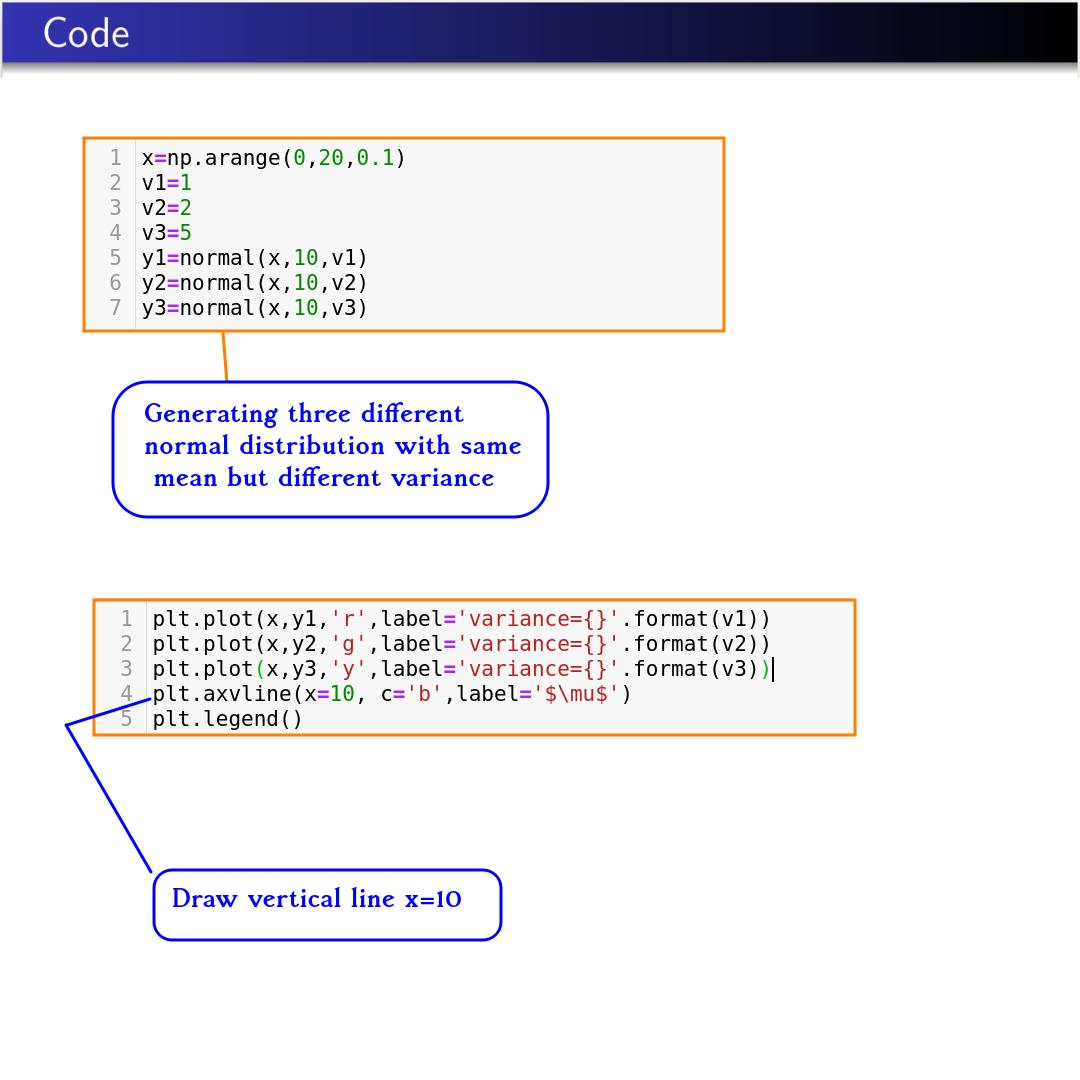
\includegraphics[scale=0.3]{4}
\end{center}
\end{frame}


\begin{frame}
\begin{center}
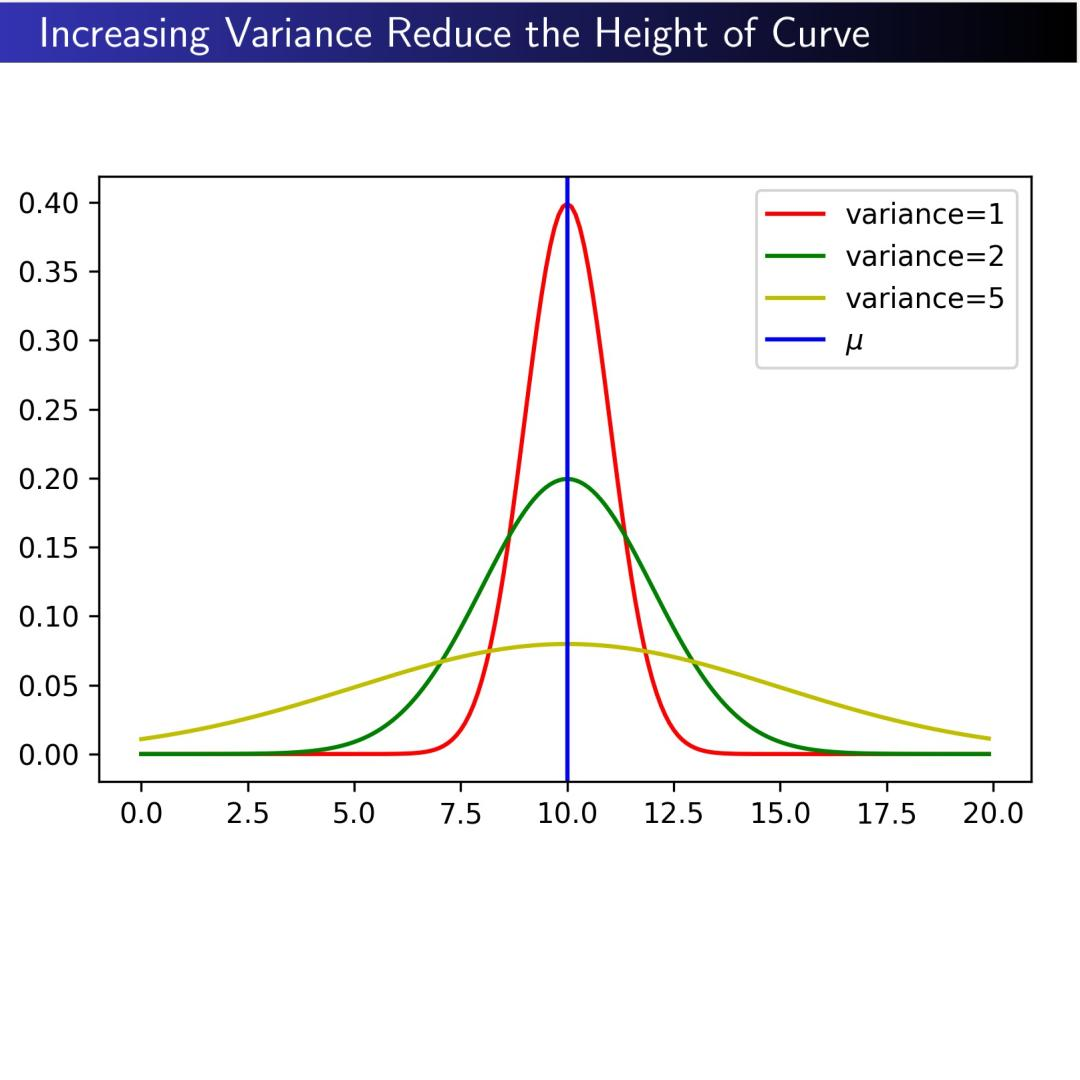
\includegraphics[scale=0.3]{5}
\end{center}
\end{frame}

\begin{frame}
\begin{center}

\includegraphics[scale=0.7]{6}
\end{center}
\end{frame}

\begin{frame}
\begin{center}
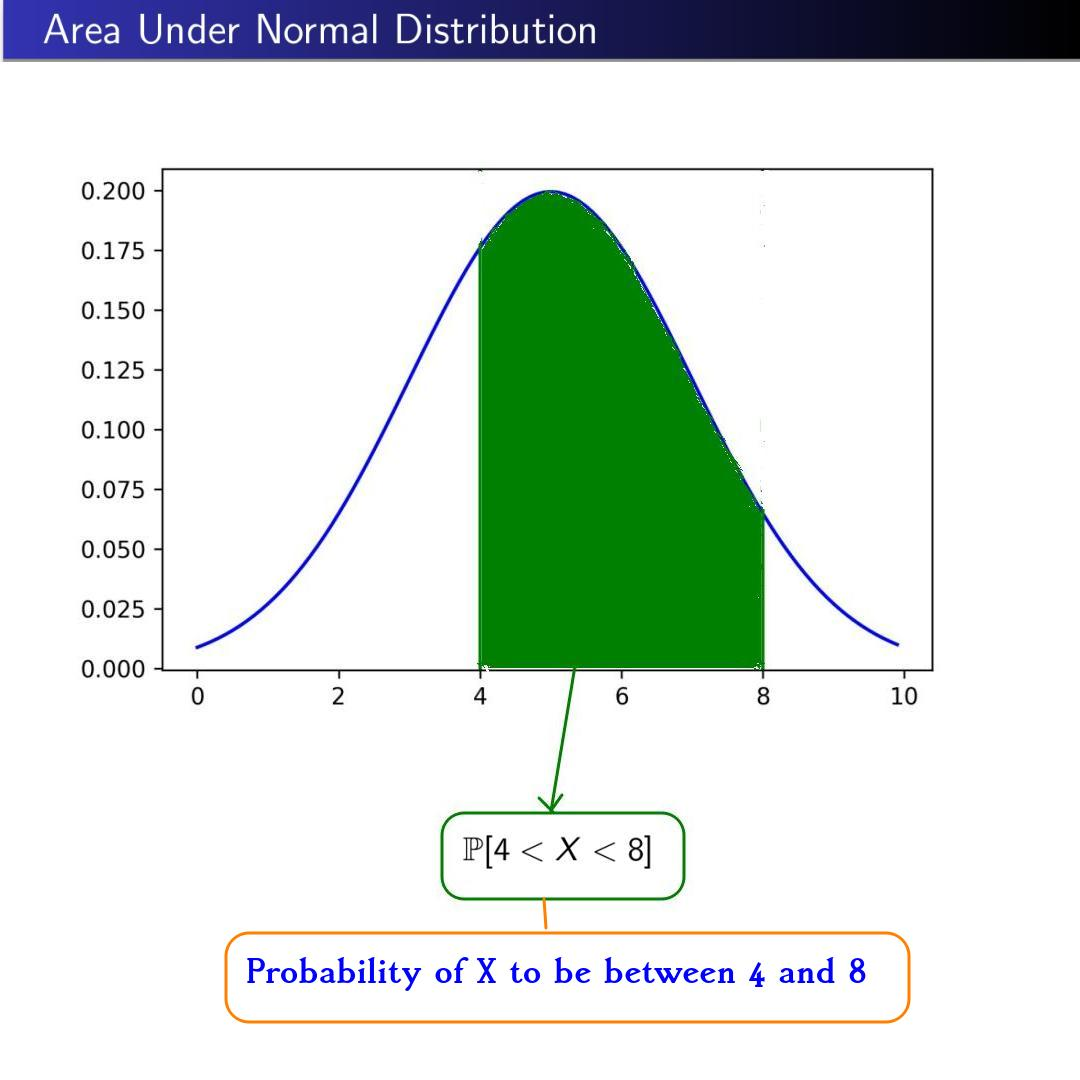
\includegraphics[scale=0.3]{7}
\end{center}
\end{frame}

\begin{frame}
\frametitle{scipy}
\begin{center}
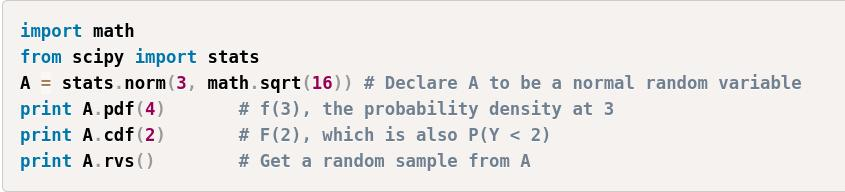
\includegraphics[scale=0.6]{scipy}
\end{center}
\end{frame}


\begin{frame}
\begin{center}

\includegraphics[scale=0.3]{./pictures/2}
\end{center}
\end{frame}


\begin{frame}
\begin{center}

\includegraphics[scale=0.3]{./pictures/3}
\end{center}
\end{frame}


\begin{frame}
\begin{center}
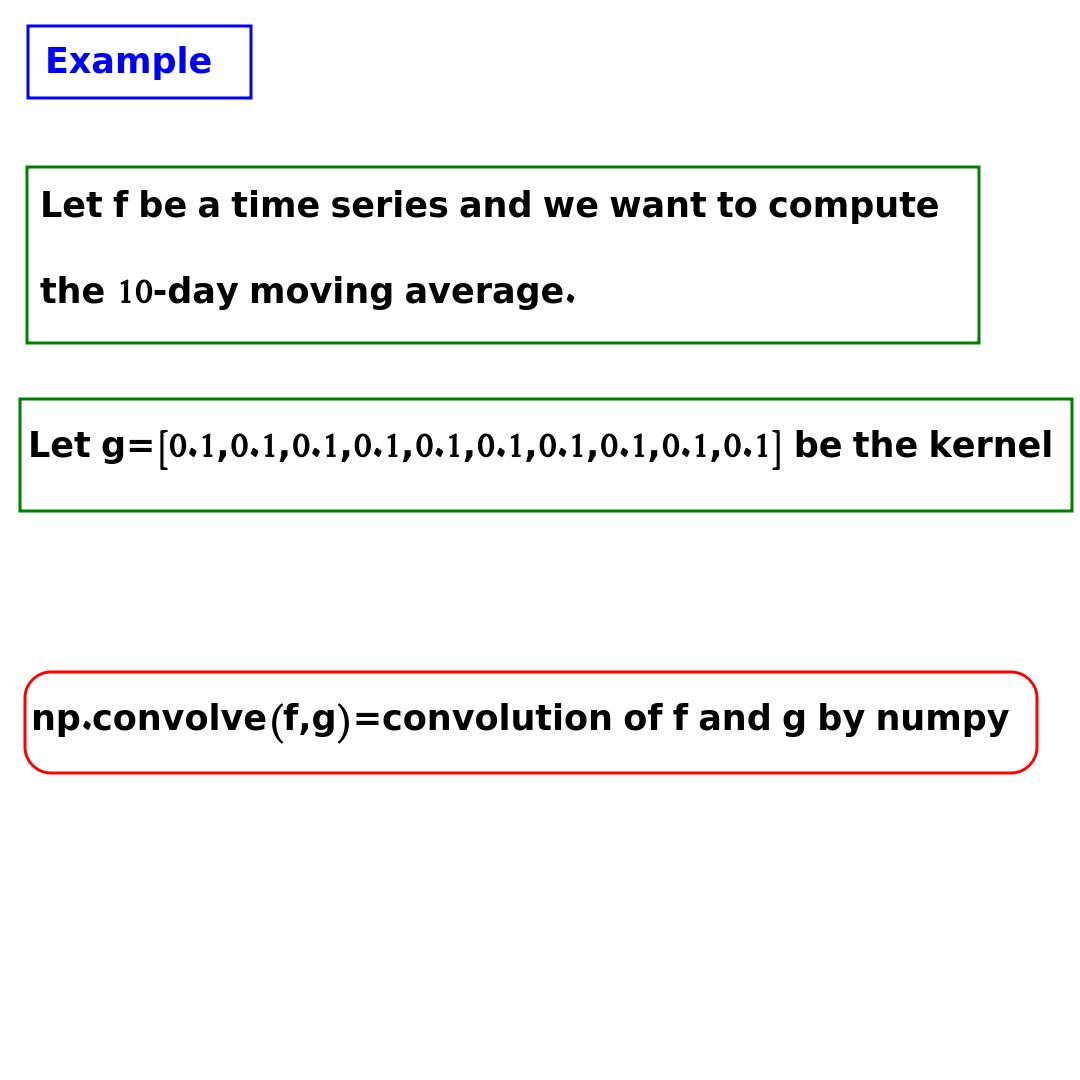
\includegraphics[scale=0.3]{./pictures/4}
\end{center}
\end{frame}


\begin{frame}
\begin{center}
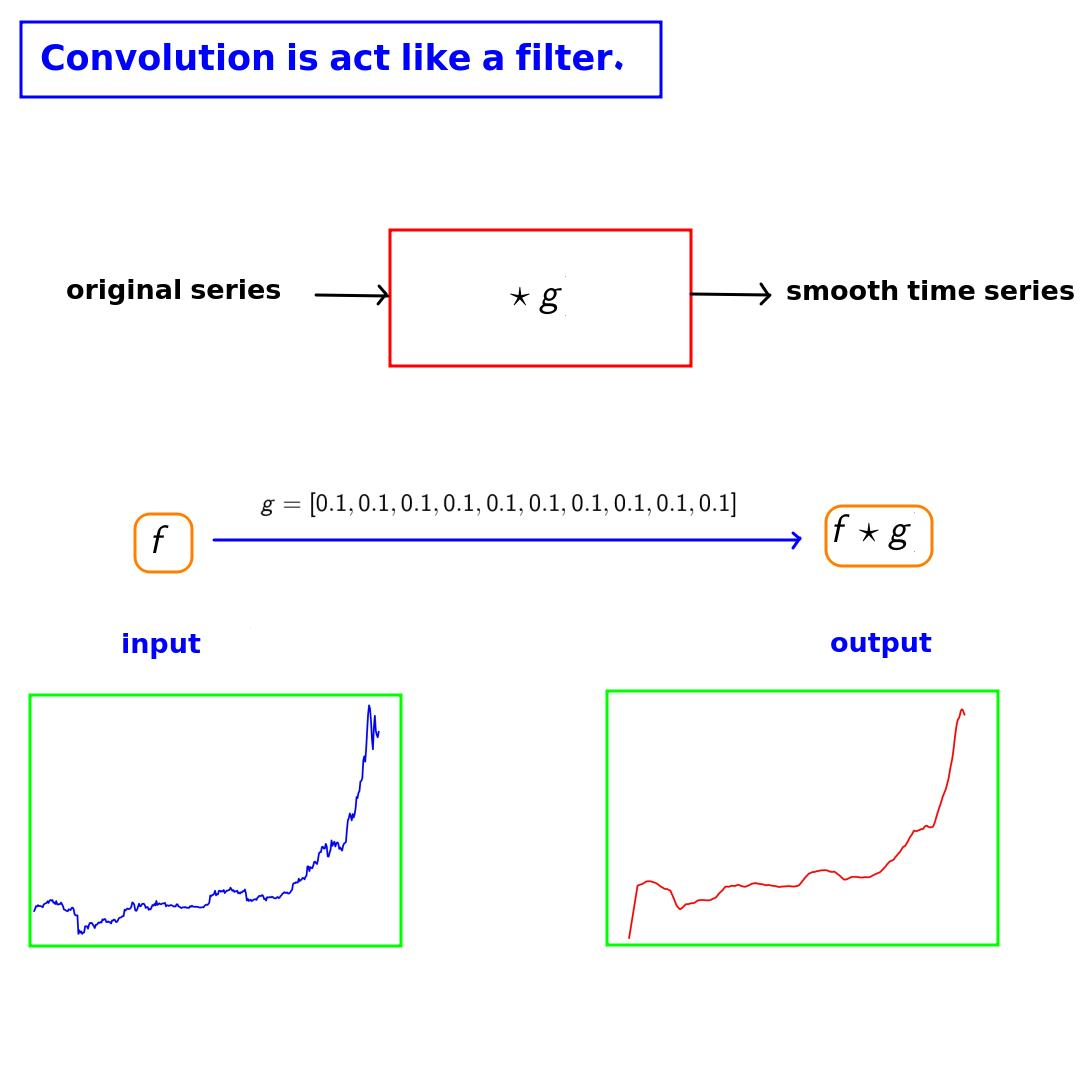
\includegraphics[scale=0.3]{./pictures/5}
\end{center}
\end{frame}


\begin{frame}
\begin{center}

\includegraphics[scale=0.3]{./pictures/6}
\end{center}
\end{frame}


\begin{frame}{}
  \centering \Huge
  \emph{Thank You}
\end{frame}

\end{document}

